% !TeX root = ../main.tex

\chapter{西瓜种植}

本章节设计了一种西瓜种植方案...
旨在简化种植的工作流程,同时...

\section{传统种植方案}

...

\subsection{西瓜种植对比实验}

...

\subsubsection{实验设计}

JSON 代码插入示例:

\begin{lstlisting}[language=json]
{
  "scene": {
    "characters": [
      {
        "avatar": "http://placeimg.com/640/480",
        "name": "Jonathan Mitchell Jr."
      },
      {
        "avatar": "http://placeimg.com/640/480",
        "name": "Jerry Torp Sr."
      }
    ],
    "dialog": {
      "text": "Quia quia eos ut assumenda quos. Est voluptate officia consequatur sint assumenda natus. ..."
    }
  }
}
\end{lstlisting}

XML 代码插入示例:

\begin{lstlisting}[language=XML]
  <?xml version="1.0" encoding="UTF-8" standalone="yes"?>
  <scene>
    <characters>
      <avatar>http://placeimg.com/640/480</avatar>
      <name>Jonathan Mitchell Jr.</name>
    </characters>
    <characters>
      <avatar>http://placeimg.com/640/480</avatar>
      <name>Jerry Torp Sr.</name>
    </characters>
    <dialog>
      <text>Quia quia eos ut assumenda quos. Est voluptate officia consequatur sint assumenda natus. ...</text>
      <name>Jonathan Mitchell Jr.</name>
    </dialog>
  </scene>
\end{lstlisting}

...

\subsubsection{实验结果及分析}

表格示例:

\begin{table}
  \centering
  \caption{JSON VS XML 读取解析性能(Chrome V8)}
  \begin{tabular}{l|ccc}
    \toprule
    方法                       & 每秒操作次数 &  误差率     & 相对落后比例\\
    \midrule
    JSON.parse                & 28 ops/s   & \pm4.36\% &  0\% \\
    xml2js.parseString        & 12 ops/s   & \pm4.16\% &  65.52\% \\
    xml2js.parseStringPromise & 10 ops/s   & \pm6.23\% &  68.97\% \\
    \bottomrule
  \end{tabular}
  \label{tab:json-vs-xml}
\end{table}

柱状图示例:

\begin{figure}[htb]
  \centering
  \begin{minipage}{.5\textwidth}
    \centering
  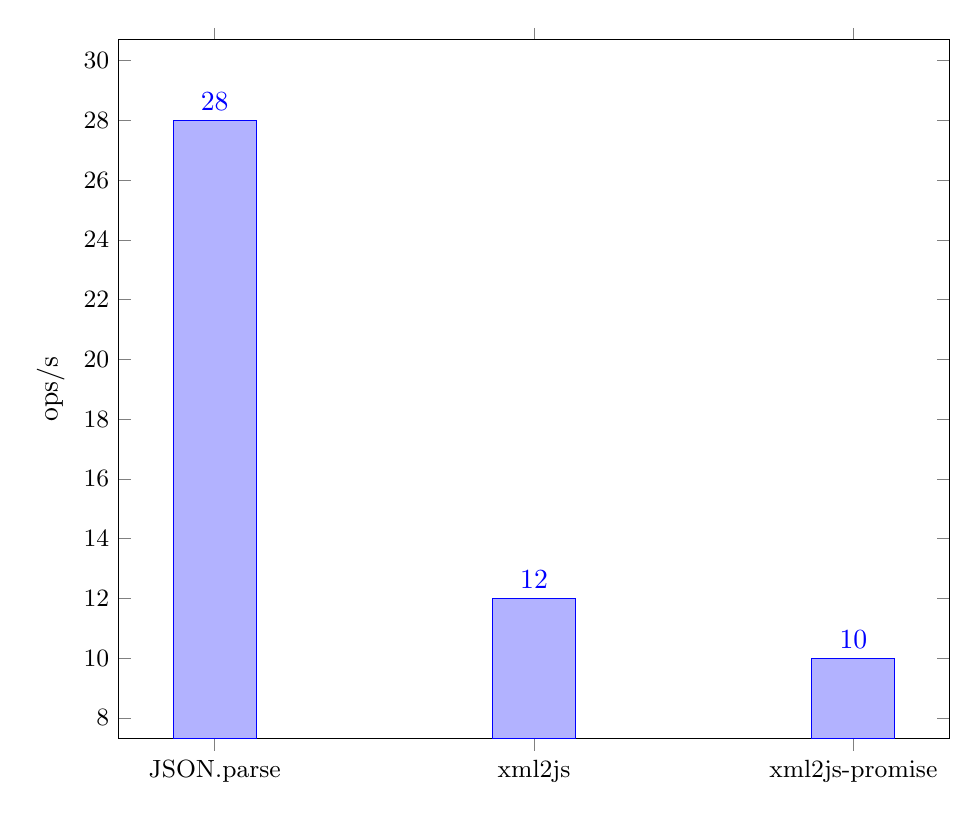
\begin{tikzpicture}
    \begin{axis}
    [
      width=\textwidth,
        bar width=30pt,
        ybar,
        enlargelimits=0.15,
        ylabel={ops/s}, % ylabel 必须在# 符号之前。
        xlabel={},
        symbolic x coords={JSON.parse, xml2js, xml2js-promise}, % 这些是 x 轴坐标的规范。
        xtick=data,
         nodes near coords, % 此命令用于提及特定条形顶部的 y 轴点。
        nodes near coords align={vertical},
        tick label style={font=\small}  
        ]
        \addplot coordinates {(JSON.parse,28) (xml2js,12) (xml2js-promise,10)};
    \end{axis}
  \end{tikzpicture}
    \label{fig:test1}
  \end{minipage}%
  \begin{minipage}{.5\textwidth}
    \centering
  \begin{tikzpicture}
    \begin{axis}
    [
      width=\textwidth,
        bar width=30pt,
        ybar,
        enlargelimits=0.15,
        ylabel={误差率$\pm\%$}, % ylabel 必须在# 符号之前。
        xlabel={},
        symbolic x coords={JSON.parse, xml2js, xml2js-promise}, % 这些是 x 轴坐标的规范。
        xtick=data,
         nodes near coords, % 此命令用于提及特定条形顶部的 y 轴点。
        nodes near coords align={vertical},
        tick label style={font=\small}  
        ]
        \addplot[red, fill=red!40] coordinates {(JSON.parse,4.36) (xml2js,4.16) (xml2js-promise,6.23)};
    \end{axis}
  \end{tikzpicture}
    \label{fig:test2}
  \end{minipage}

  \caption{JSON VS XML 读取解析性能对比}
  \label{fig:json-vs-xml}
\end{figure}

引用可以使用 \verb!\ref! 的方式。

写成如表~\ref{tab:json-vs-xml},将会自动编号。

\section{西红柿炒鸡蛋}

普通文本代码示例:

\begin{lstlisting}[]
  好久不见,你去哪儿啦?

  江湖。

  江湖在什么地方?

  我指给你看………………
\end{lstlisting}


\section{一些语法帮助}

\subsection{枚举示例}

有序号枚举示例:

\begin{enumerate}
  \item 新年快乐
  \item 万事如意
  \item 心想事成
\end{enumerate}

没序号的:

\begin{itemize}
  \item 新年快乐
  \item 万事如意
  \item 心想事成
\end{itemize}

\verb!\backslash! 表示反斜杠,\backslash。


\begin{lstlisting}[]
> 好久不见,你去哪儿啦?
>
> 江湖。
>
> 江湖在什么地方?
>
> 我指给你看………………
\end{lstlisting}

树节点画法:

\begin{figure}[htb]
  \centering
  \begin{minipage}[t]{.4\textwidth}
    \centering
    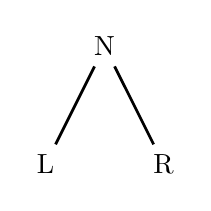
\begin{tikzpicture}[
      line width = 1pt,
      N/.style={draw,circle},
      L/.style={draw,circle, sibling distance=3cm, level distance=1cm},
      R/.style={sibling distance=1.5cm, level distance=0.8cm}]
      \node {N}
      child {node {L}}
      child {node {R}};
    \end{tikzpicture}
  \end{minipage}
  \begin{minipage}[t]{.4\textwidth}
    \centering
    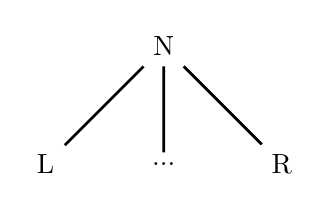
\begin{tikzpicture}[
      line width = 1pt,
      N/.style={draw,circle},
      L/.style={draw,circle, sibling distance=3cm, level distance=1cm},
      R/.style={sibling distance=1.5cm, level distance=0.8cm}]
      \node {N}
      child {node {L}}
      child {node {...}}
      child {node {R}};
    \end{tikzpicture}
  \end{minipage}
  \caption{节点示意图}
  \label{fig:unist-node}
\end{figure}

\begin{figure}[htb]
\centering
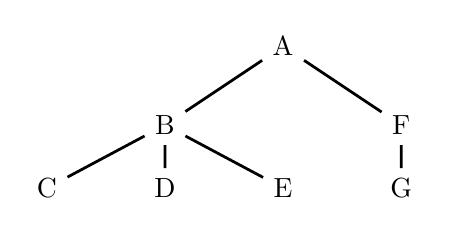
\begin{tikzpicture}[
  line width = 1pt,
  level 1/.style={sibling distance=3cm, level distance=1cm},
  level 2/.style={sibling distance=1.5cm, level distance=0.8cm}]
\node {A}
child {node {B}
  child {node {C}}
  child {node {D}}
  child {node {E}}
}
child {node {F}
  child {node {G}}
};
\end{tikzpicture}
\caption{多节点语法树示意图} \label{fig:unist-tree-example}
\end{figure}


\subsection{实验设计}

...

\subsection{实验结果及分析}

。。。

\section{本章小结}

本章第一节回顾了...

发现还是直接买最方便。
